\chapter{اتّصال به تلفن ثابت}
\label{pstnPart}
\setlatintextfont{Times New Roman}
یکی از مسائل مهم در پیاده\nf سازی \lr{clearwater}، ارتباط این معماری با سایر شبکه\nf ها نظیر \lr{PSTN} است. با اتّصال \lr{IMS} به \lr{PSTN} یا \lr{ISDN}\RTLfootnote{سرواژه\nf ی عبارت \lr{Integrated Service Digital Network} و به معنای شبکه\nf ی سرویس یکپارچه\nf ی دیجیتال}، کابران تلفن ثابت و کاربران \lr{IMS} می\nf توانند با یکدیگر تماس تلفنی برقرار کنند. شبکه\nf های \lr{PSTN}، ساختاری قدیمی و آنالوگ دارند امّا شبکه\nf های \lr{ISDN}، ساختاری جدید و دیجیتال دارند. برای اتّصال با \lr{PSTN} یا \lr{ISDN}، باید از \lr{SIP trunk} استفاده کرد. \lr{SIP trunk}، پیام\nf های کنترلی مربوط به \lr{SIP} را به پیام\nf های کنترلی مورد استفاده در خطوط تلفن ثابت تبدیل می\nf کند. از آنجایی\nf که سرویس \lr{VOIP} و سرویس \lr{IMS}، هر دو از پروتکل \lr{SIP} استفاده می\nf کنند، می\nf توان از \lr{SIP trunk}هایی که برای اتّصال سرویس \lr{VOIP} به تلفن ثابت استفاده می\nf شود، برای \lr{IMS} نیز استفاده کرد.


\section{روش\nf های استفاده از \lr{SIP trunk}}
\subsubsection{استفاده از \lr{SIP trunk} تأمین\nf کنندگان \lr{VOIP} }

روش\nf های متفاوتی برای استفاده از \lr{SIP trunk} و اتّصال \lr{IMS} به شبکه\nf ی تلفن ثابت وجود دارد. روش اوّل، استفاده از \lr{SIP trunk} ایجادشده توسّط سایر تأمین\nf کنندگان سرویس \lr{VOIP} است. از آنجایی\nf که بسیاری از ارائه\nf کنندگان سرویس \lr{VOIP}، از طریق \lr{SIP trunk} به شبکه\nf ی تلفن ثابت دسترسی دارند، می\nf توان از شبکه\nf ی آن\nf ها به عنوان یک درگاه برای ارتباط با تلفن ثابت، بهره\nf مند شد. 

پیشنهاد \lr{clearwater}، استفاده از تأمین\nf کننده\nf ای به نام \lr{voxbone} است. در مستندات \lr{clearwater}، نحوه\nf ی اتّصال به \lr{voxbone} با استفاده از رابط\nf های برنامه\nf نویسی اپلیکیشن آورده شده است. با اتّصال به \lr{voxbone} می\nf توان از \lr{SIP trunk} پیاده\nf سازی\nf شده\nf ی آن برای ارتباط با تلفن ثابت استفاده کرد. \lr{voxbone}، در بیش از ۹۰ کشور دنیا سرویس ارائه می\nf کند؛ امّا از آنجایی\nf که ایران، جزو کشورهای تحت پوشش این سرویس نیست، استفاده از این روش مقدور نمی\nf باشد\cite{webvoxbone}\cite{webcw}. 

با وجود اینکه \lr{voxbone}، تنها ارائه\nf کننده\nf ی سرویس \lr{VOIP} است که توسّط توسعه\nf دهندگان تیم \lr{clearwater}، مورد آزمایش و ارزیابی قرار گرفته\nf است، امّا بدیهی است که می\nf توان از سایر ارائه\nf کنندگان نیز برای این کار استفاده کرد. به عنوان مثال، این امکان وجود دارد که با اتّصال \lr{IMS} به سرویس \lr{VOIP} دانشگاه صنعتی اصفهان، از \lr{SIP trunk} پیاده\nf سازی\nf شده توسّط این سرویس استفاده کرد.

\subsubsection{پیادهسازی \lr{SIP trunk}} 
\lr{SIP trunk}های تجاری به نام درگاه وویپ(\lr{VOIP}) وجود دارند و می\nf توان از آن\nf ها استفاده کرد. شرکت \lr{Sangoma}، یکی از تولیدکنندگان بزرگ این درگاه\nf ها است و سرویس \lr{VOIP}  دانشگاه صنعتی اصفهان نیز، از محصولات همین شرکت برای ایجاد \lr{SIP trunk} استفاده می\nf کند. متأسّفانه، این درگاه\nf ها، قیمت بالایی(چند میلیون تومان) دارند. لذا، راه\nf حل جایگزین، طرّاحی و ساخت \lr{SIP trunk} است.  

طرّاحی \lr{SIP trunk} در دو بخش نرم\nf افزاری و سخت\nf افزاری صورت می\nf گیرد. در پروژه\nf ی کارشناسی دانشجویان\RTLfootnote{بخش نرم\nf افزاری توسّط آقای حسین خلیلیان و بخش سخت\nf افزاری توسّط آقای احمدرضا بدیهی انجام شده است.} دانشکده\nf ی برق و کامپیوتر تحت عنوان "طرّاحی و پیاده\nf سازی رابط شبکه\nf ی \lr{\lr{VOIP}} و \lr{PSTN}"، بخش نرم\nf افزاری و سخت\nf افزاری \lr{SIP trunk} طرّاحی و ساخته شده است. بخش نرم\nf افزاری شامل سه بخش است:
\begin{itemize}
\item پیاده\nf سازی یک نرم\nf افزار برای ایجاد تماس تلفنی
\item توسعه\nf ی نرم\nf افزار برای دریافت و پاسخ به تماس تلفنی
\item نرم\nf افزار ارسال و دریافت صدا
\end{itemize}
 سخت\nf افزار \lr{SIP trunk} نیز به طور کلّی شامل پنج قسمت است:
 \begin{itemize}
 \item مدار  \lr{Off Hook}\RTLfootnote{زمانی که خط تلفن اشتغال است.} تلفن
 \item مدار تشخیص زنگ تلفن
 \item مدار دریافت و ارسال صوت
 \item مدار راه\nf انداز \lr{USB}
 \item مدار مربوط به میکروکنترلر
 \end{itemize}
 با استفاده از سخت\nf افزار و نرم\nf افزار موردنظر، می\nf توان شبکه\nf ی \lr{VOIP} را به شبکه\nf ی تلفن ثابت متّصل کرد. برای اتّصال \lr{SIP trunk}، باید آدرس \lr{IP} اینترفیسی که آن را به سرور مربوطه متّصل می\nf کند، در پیکربندی سرور وارد شود. در بعضی از سیستم\nf ها، نیاز است که شماره\nf ی پورت مورد استفاده نیز مشخّص شود. برای اطّلاعات بیشتر، به گزارش پروژه\nf ی مذکور مراجعه شود.

\section{اتّصال \lr{SIP trunk} به \lr{IMS}}

برای ارتباط \lr{clearwater} با \lr{SIP trunk}، باید المان موردنیاز برای این کار، به معماری \lr{clearwater} اضافه شود و در پیکربندی سایر المان\nf های مربوطه نیز، تغییراتی ایجاد شود. المان \lr{IBCF}، رابطِ بین پیاده\nf سازی \lr{clearwater} و \lr{SIP trunk} است. المان \lr{IBCF}
توسّط \lr{clearwater} پیاده\nf سازی شده است، بسیاری از کارکردهای موردنیاز را تأمین می\nf کند؛ امّا بعضی کارکردها مانند پنهان\nf سازی توپولوژی شبکه\nf ی داخلی \lr{IMS}، هنوز پیاده\nf سازی نشده\nf اند. برای استفاده از \lr{IBCF}، حدّاقل باید یک نود \lr{IBCF} را نصب و پیکربندی کرد. سپس باید المان \lr{ENUM} را برای نگاشت شماره\nf ی تلفن، پیکربندی کرد. سپس باید پیکربندی مربوط به مسیریابی \lr{BGCF} را که در نود \lr{Sprout} قرار دارد، انجام داد. شکل \ref{siptrunk}، نحوه\nf ی اتّصال تلفن ثابت به شبکه\nf ی \lr{IMS} را نشان می\nf دهد. مطالب این بخش، بر اساس مستندات پروژه\nf ی \lr{clearwater}\cite{webcw} نوشته شده\nf اند.

\begin{figure}[h]
\centering
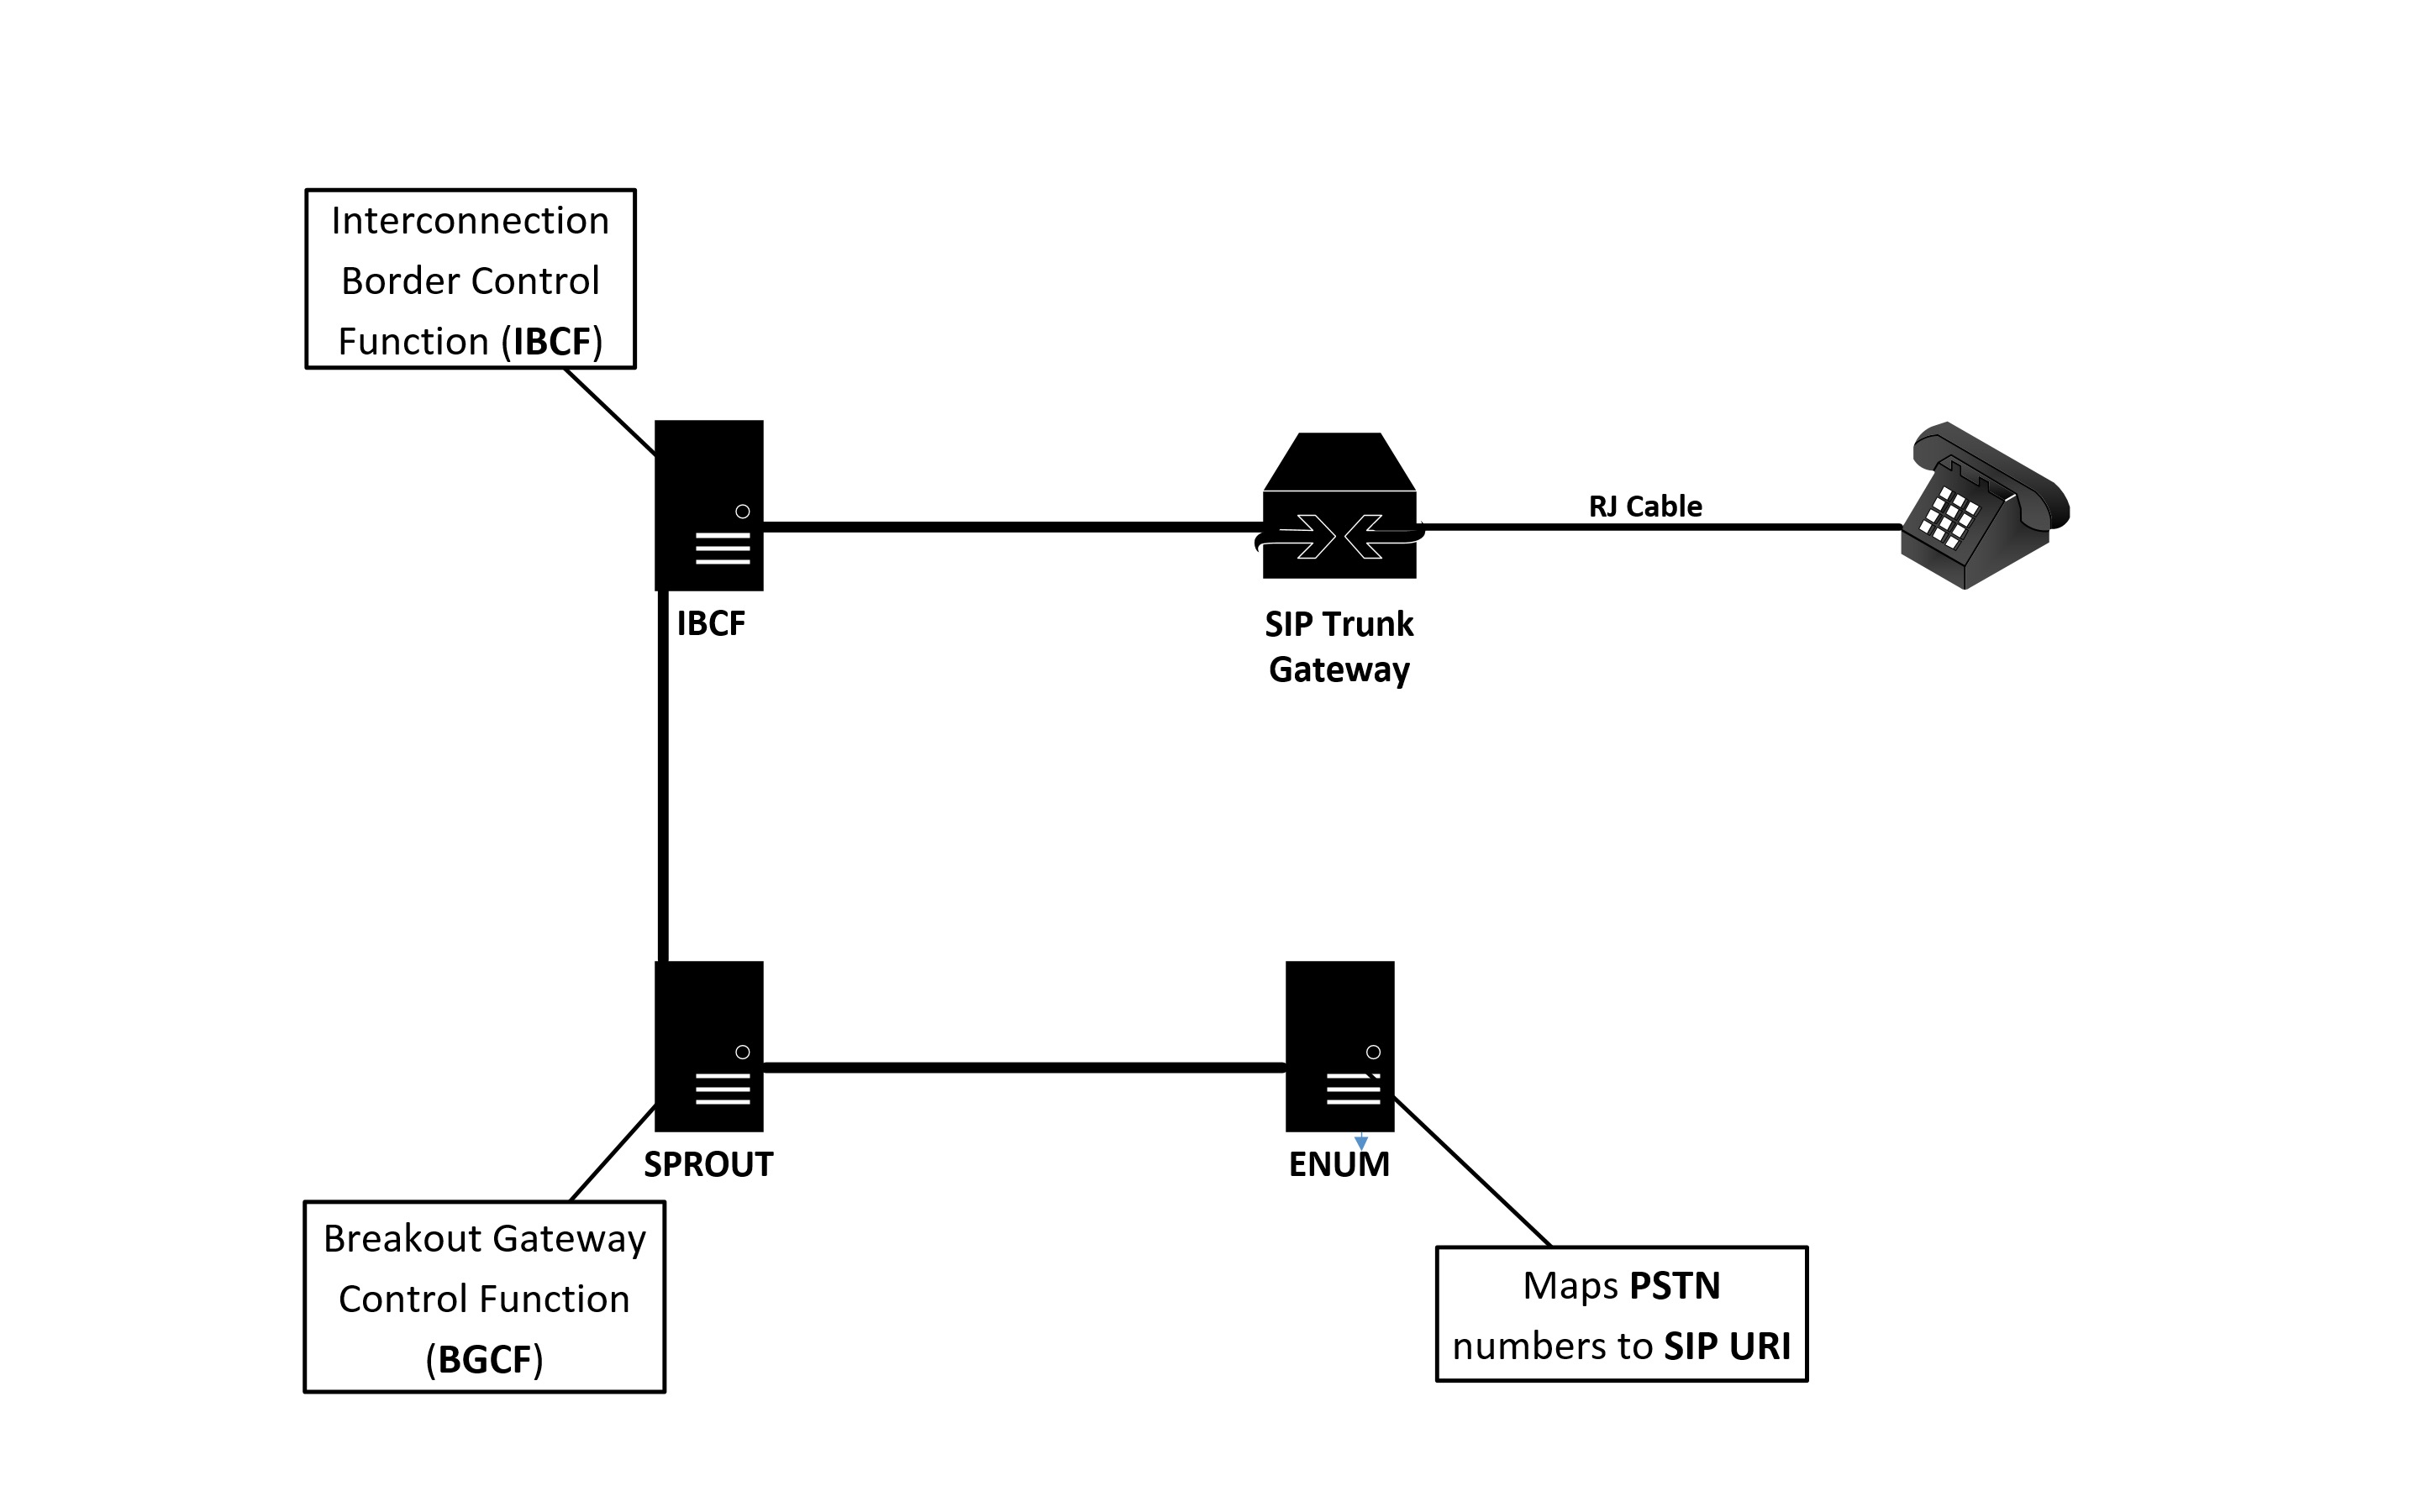
\includegraphics[width=\textwidth]{siptrunk}
\caption{نحوه\nf ی ارتباط \lr{SIP trunk} با \lr{IMS} و اتّصال به \lr{PSTN}}
\label{siptrunk}
\end{figure}

\subsection{نصب و پیکربندی \lr{IBCF}}
نصب \lr{IBCF}، مانند نصب دستی نود \lr{Bono} می\nf باشد. بنابراین، ابتدا باید نود \lr{Bono} را نصب کرد. روش نصب نودهای معماری \lr{clearwater}، در مستندات این پروژه و در قسمت نصب به صورت دستی بر روی سیستم\nf های مجزّا(\lr{manual install}) آورده\nf شده است. در این قسمت، نصب نود \lr{Bono} به\nf صورت جداگانه بیان شده است.
\subsubsection{پیش\nf نیازها}
ابتدا باید نسخه\nf ی سرور 64 بیت سیستم عامل اوبونتوی \lr{14.04} را بر روی یک ماشین نصب کرد. حدّاقل سخت\nf افزار مورد نیاز برای راه\nf اندازی این نود، مانند سخت\nf افزار لازم برای پیاده\nf سازی\nf های یکپارچه و در مقیاس کوچک(بخش \ref{yekparchePart}) است. همچنین، نیاز است که یک آدرس \lr{IP} عمومی\RTLfootnote{به\nf جای \lr{IP} آدرس عمومی، می\nf توان یک آدرس \lr{IP} در شبکه\nf ی محلّی خود به ماشین اختصاص داد، به طوری که از تمام نقاط شبکه\nf ی داخلی بتوان به آن آدرس \lr{IP} دسترسی داشت. در این صورت، آدرس \lr{IP} خصوصی که برای ارتباط نودهای \lr{clearwater} مورد استفاده قرار می\nf گیرد، می\nf تواند آدرس پشت \lr{NAT} در همان شبکه\nf ی محلّی باشد.} و یک آدرس \lr{IP} خصوصی به ماشین اختصاص داده شود. 

\subsubsection{اضافه کردن مخازن \lr{clearwater}}
برای ایجاد فایل موردنظر، دستور زیر را وارد کنید و عبارت \lr{\textcolor{black}{deb http://repo.cw-ngv.com/stable binary/}} را به فایل موردنظر اضافه کنید.
\begin{latin}
\noindent sudo nano /etc/apt/source.list.d/clearwater.list
\end{latin}
\noindent سپس با استفاده از دستور زیر، کلیدهایِ امضای مورد استفاده توسّط سرور \lr{clearwater} را نصب کنید.
\begin{latin}
\noindent curl -L http://repo.cw-ngv.com/repo\_ key | sudo apt-key add -
\end{latin} 
\noindent با استفاده از دستور زیر، اثر انگشت\RTLfootnote{\lr{Fingerprint}} را چک کنید. 
\begin{latin}
\noindent sudo apt-key finger
\end{latin}
\noindent خروجی دستور فوق، باید شامل عبارات زیر باشد:
\begin{latin}
\setlength{\parindent}{0ex}
pub\hspace{1cm} 4096R/22B97904 2013-04-30 \newline
Key fingerprint = 9213 4604 DE32 7DF7 FEB7  2026 111D BE47 22B9 7904

uid\hspace{1cm} Project Clearwater Maintainers <maintainers@projectclearwater.org>

sub\hspace{1cm} 4096R/46EC5B7F 2013-04-30
\end{latin}
\noindent پس از انجام موفقیّت\nf آمیز مراحل فوق، دستور زیر را اجرا کنید.
\begin{latin}
\noindent sudo apt-get update
\end{latin}

\subsubsection{تنظیمات دیوار آتش}
نودهای \lr{clearwater}، از طریق پروتکل \lr{IP}، با یکدیگر ارتباط برقرار می\nf کنند. برای این ارتباط، از پورت\nf های مختلفی استفاده می\nf شود. لازم است که در تنظیمات دیوار آتش، اجازی استفاده از این پورت\nf ها داده\nf شود. برای برقراری ارتباط \lr{SSH}، لازم است که پورت \lr{TCP/22} باز باشد. برای برقراری سیگنالینگ\nf های \lr{STUN}، لازم است که پورت \lr{3478} هم برای \lr{TCP} و هم برای \lr{UDP} باز باشد. برای سیگنالینگ\nf های \lr{SIP}، پورت\nf های \lr{TCP/5062} و \lr{TCP/5060} و \lr{UDP/5060} مورد استفاده قرار می\nf گیرد. همچنین، برای فورواردینگ \lr{RTP}، نیاز است که پورت\nf های \lr{UDP/32768-65535} باز باشند. برای بازکردن پورت\nf های مذکور، دستورات زیر را اجرا کنید. 

\begin{latin}
\setlength{\parindent}{0ex}
sudo ufw allow 22,3478,5060,5062/tcp

sudo ufw allow 3478,5060,32768:65535/udp
\end{latin} 

\subsubsection{پیکربندی محلّی}
قبل از نصب نود، نیاز است که پیکربندی اوّلیه برای ارتباط با سایر نودها انجام شود. برای این کار، با استفاده از دستور شماره \lr{1}، فایل پیکربندی محلّی(\lr{local\_ config}) را ایجاد کنید. در صورت عدم وجود پوشه\nf ی موردنظر، ابتدا دستورات  \lr{2} و \lr{3} را اجرا کرده و سپس دستور \lr{1} را اجرا کنید.
\begin{latin}
\setlength{\parindent}{0ex}
1. sudo nano /etc/clearwater/local\_ config

2. cd  /etc

3. mkdir clearwater
\end{latin}

پس از ایجاد فایل موردنظر، اطّلاعات زیر را وارد آن کنید. در عبارت زیر، به\nf جای \lr{<privateIP>}، آدرس \lr{IP} خصوصی ماشین و به\nf جای \lr{publicIP}، آدرس \lr{IP} عمومی ماشین را قرار دهید. به\nf جای عبارت \lr{hostname} نیز آدرس \lr{IP} عمومی را قرار دهید. به\nf جای عبارت \lr{<comma separated list of private IPs>}، باید آدرس \lr{IP} خصوصی تمام نودهای معماری \lr{clearwater} را قرار دهید و بین این آدرس\nf ها، به وسیله\nf ی علامت '\lr{,}'، فاصله ایجاد شود. به\nf عنوان مثال، عبارت \lr{10.0.0.1,10.0.0.2,10.0.0.3,10.0.0.4,10.0.0.5} می\nf تواند یک نمونه از مقداردهی برای \lr{etcd\_ cluster} باشد.

\nf 
\begin{latin}
\setlength{\parindent}{0ex}
local\_ ip=<privateIP>

public\_ ip=<publicIP>

public\_ hostname=<hostname>

etcd\_ cluster="<comma separated list of private IPs>"
\end{latin}

\subsubsection{نصب \lr{Bono}}
برای نصب نود \lr{Bono}، دستورات زیر را اجرا کنید:
\begin{latin}
\setlength{\parindent}{0ex}
sudo DEBIAN\_ FRONTEND=noninteractive apt-get install Bono restund --yes

sudo DEBIAN\_ FRONTEND=noninteractive apt-get install clearwater-management --yes

\end{latin}

\subsubsection{پیکربندی \lr{IBCF}}
پس از نصب نود \lr{Bono}، باید \lr{IBCF} را پیکربندی کرد تا \lr{SIP trunk} یا \lr{SIP trunk}های\RTLfootnote{می\nf توان هم\nf زمان از چند \lr{SIP trunk} استفاده کرد} مورد استفاده را به رسمیت بشناسد. برای این کار، باید فایل \lr{user\_ settings} را ویرایش کنید. این فایل، در پوشه\nf ی \lr{/etc/claerwater} قرار دارد. در صورت موجود نبودن این فایل، آن را ایجاد کنید. با اجرای دستور زیر، فایل موردنظر باز می\nf شود(در صورت موجود نبودن، ایجاد می\nf شود).
\begin{latin}
\noindent sudo nano /etc/clearwater/user\_ settings
\end{latin}

\noindent سپس، آدرس \lr{IP} مربوط به \lr{SIP trunk} یا \lr{SIP trunk}های خود را به عنوان \lr{trusted\_ peers} معرّفی کنید. برای این کار، به\nf جای \lr{<trunk IP address>}، آدرس \lr{IP} مربوطه را قرار دهید.

\begin{latin}
\noindent trusted\_ peers="<trunk 1 IP address>,<trunk 2 IP address>, ..."
\end{latin}
\noindent پس از انجام این پیکربندی، نود \lr{Bono} را با دستور زیر، دوباره شروع\RTLfootnote{\lr{Restart}} کنید.
\begin{latin}
\noindent service stop bono
\end{latin}

\nf 

\subsection{پیکربندی \lr{ENUM}}
سیستم \lr{ENUM}، برای نگاشت شماره تلفن\nf های \lr{PSTN} به \lr{SIP URI}\RTLfootnote{سرواژه\nf ی عبارت \lr{Uniform Resource Identifier} و روشی برای نمایش آدرس\nf های \lr{SIP} است. این آدرس\nf ها به شکل \lr{user@domain.tdl} می\nf باشند. به\nf عنوان مثال، \lr{6505551234@example.com} یک \lr{SIP URI} است. } مورد استفاده قرار می\nf گیرد. این کار، با استفاده از بایگانی\RTLfootnote{\lr{Record}} \lr{NAPTR}\RTLfootnote{کوتاه\nf شده\nf ی عبارت \lr{Name Authority Pointer} است. \lr{NAPTR} گونه\nf ای از بایگانی منابع در سیستم نام دامنه\nf ی اینترنت است. بایگانی\nf های \lr{NAPTR} بیشتر در اپلیکیشن\nf های \lr{VOIP} مورد استفاده قرار می\nf گیرند و عموماً کار نگاشت آدرس سرورها و کاربران را در پروتکل \lr{SIP} انجام می\nf دهند.}  سیستم نام دامنه صورت می\nf گیرد. علّت استفاده از \lr{NAPTR}، پشتیبانی \lr{Sprout} از این نوع بایگانی است. بازه\nf ی شماره تلفن\nf هایی که قرار است از طریق \lr{SIP trunk} مسیریابی شوند، باید در پیکربندی \lr{ENUM} وارد شوند. از آنجایی\nf که \lr{ENUM}، پیکربندی\nf ها و نگاشت\nf های مخصوص به خود را دارد، نیاز است که ابتدا بخش \lr{ENUM Guid} در \cite{webenum} مطالعه شود. پس از کسب اطّلاعات لازم در مورد \lr{ENUM}، می\nf توان نحوه\nf ی نگاشت شماره تلفن\nf ها را وارد پیکربندی این سیستم کرد.


\subsection{پیکربندی \lr{BGCF}}
فایل پیکربندی \lr{BGCF} به نام \lr{bgcf.json} در پوشه\nf ی \lr{/etc/clearwater} قرار دارد. ابتدا باید با دستور شماره \lr{4}، یک کپی از این فایل را ایجاد کرده و سپس فایل کپی\nf شده را ویرایش کنید. فایل کپی\nf شده در پوشه\nf ی \lr{clearwater-config-manager} قرار می\nf گیرد. برای ویرایش فایل مورد نظر، از دستورات \lr{5} و \lr{6} استفاده کنید. در دستور شماره\nf ی \lr{6}، به\nf جای عبارت \lr{<user>}، نام کاربری خود در سیستم عامل را قرار دهید.
\begin{latin}
\setlength{\parindent}{0ex}
4. clearwater-config  downlaod  bgcf\_ json \\
5. cd /home/<user>/clearwater-config-manager/<user> \\
6. sudo nano bgcf.json \\
\end{latin}

فایل \lr{bgcf.json} دو نوع نگاشت را ذخیره می\nf کند. در نوع اوّل، آدرس \lr{IP} مربوط به \lr{SIP trunk} و نام\nf های دامنه را به \lr{SIP URI}های \lr{IBCF} نگاشت می\nf کند. در نوع دوّم، شماره\nf های تلفن را به \lr{SIP URI}های \lr{IBCF} تبدیل می\nf کند. برای هر نام دامنه، \lr{IP} آدرس \lr{SIP trunk} و شماره تلفن، تنها یک مسیر می\nf تواند قرار داده شود. اگر برای  برای هر یک از موارد گفته\nf شده، بیش از یک مسیر در درنظر گرفته\nf شود، فقط اوّلین مسیر مورد استفاده قرار می\nf گیرد. فایل \lr{bgcf.json}، به فرمت \lr{JSON} است. عبارات زیر، نمونه\nf ای از جدول مسیرها می\nf باشد که به فرمت \lr{JSON} نوشته شده است.
\begin{latin}
\setlength{\parindent}{0ex}
\{\\
\hspace*{1cm}"routes" : [\\
\hspace*{1.5cm}\{\hspace{0.25cm}    "name" : "<route 1 descriptive name>",\\
\hspace*{2cm}"domain" : "<SIP trunk IP address or domain name>",\\
\hspace*{2cm}"route" : ["<IBCF SIP URI>"]\\
\hspace*{1.5cm}\},\\
\hspace*{1.5cm}\{\hspace{0.25cm}   "name" : "<route 2 descriptive name>",\\
\hspace*{2cm}"domain" : "<SIP trunk IP address or domain name>",\\
\hspace*{2cm}"route" : ["<IBCF SIP URI>", "<IBCF SIP URI>"]\\
\hspace*{1.5cm}\},\\
\hspace*{1.5cm}\{ \hspace{0.25cm}   "name" : "<route 3 descriptive name>",\\
\hspace*{2cm}"number" : "<Telephone number>",\\
\hspace*{2cm}"route" : ["<IBCF SIP URI>", "<IBCF SIP URI>"]\\
\hspace*{1.5cm}\}\\
\hspace*{1cm}]\\
\} \\
\end{latin}
\noindent بعد از اعمال تغییرات در این فایل، دستور زیر را اجرا کنید تا تغییرات لازم در نود \lr{Sprout} که المان \lr{BGCF} در آن قرار دارد، اعمال شود.
\begin{latin}
\noindent cw-config upload bgcf\_ json
\end{latin}
